%pdflatex main.tex
\documentclass[12pt]{article}
\usepackage{natbib}
\usepackage[francais]{babel}
\usepackage{natbib}
\usepackage{url}
\usepackage[utf8x]{inputenc}
\usepackage{amsmath}
\usepackage{graphicx}
\usepackage{float}
\graphicspath{{images/}}
\usepackage{amsthm}
\usepackage{parskip}
\usepackage{fancyhdr}
\usepackage{xfrac}
\usepackage{esvect}
\usepackage{vmargin}
\usepackage{gensymb}
\setmarginsrb{3 cm}{2.5 cm}{3 cm}{2.5 cm}{1 cm}{1.5 cm}{1 cm}{1.5 cm}

\title{POC}								% Title
\author{}								% Author
\date{\today}											% Date

\makeatletter
\let\thetitle\@title
\let\theauthor\@author
\let\thedate\@date
\makeatother

\pagestyle{fancy}
\fancyhf{}
\rhead{\theauthor}
\lhead{\thetitle}
\cfoot{\thepage}
\newtheorem*{rappel}{Rappel}
\newtheorem*{nota}{N.B}
\newtheorem*{req}{Remarque}
\begin{document}

%%%%%%%%%%%%%%%%%%%%%%%%%%%%%%%%%%%%%%%%%%%%%%%%%%%%%%%%%%%%%%%%%%%%%%%%%%%%%%%%%%%%%%%%%

\begin{titlepage}
	\centering
    \vspace*{0.5 cm}
    
\includegraphics[scale = 0.75 ]{logo1.png}\\[1.0 cm]	% University Logo
    \textsc{\LARGE EISTI}\\[2.0 cm]			% University Name
    \rule{\linewidth}{0.2 mm} \\[0.5 cm]
    { \huge \bfseries \thetitle}\\
    \rule{\linewidth}{0.2 mm} \\[1.5 cm]
	\textsc{\Large Projet Différencié}\\[0.5 cm]	% Course Code
	\textsc{\large ING1 GI}\\[0.5 cm]		% Course Name
	
	\begin{minipage}{0.4\textwidth}
	\centering
		\begin{center} \large
		Thomas PIZZINATO \\
		Olivier LISANDRE \\
		Ismaël L'HOSTE \\
		David RIGAUX \\
			\end{center}
			\end{minipage}~
			\begin{minipage}{0.4\textwidth}
	\end{minipage}\\[0.8 cm]
	{\large \thedate}\\[1 cm]
	\vfill
	
\end{titlepage}

%%%%%%%%%%%%%%%%%%%%%%%%%%%%%%%%%%%%%%%%%%%%%%%%%%%%%%%%%%%%%%%%%%%%%%%%%%%%%%%%%%%%%%%%%

\tableofcontents
\addtocontents{toc}{~\hfill\textbf{Page}\par}
\pagebreak

%%%%%%%%%%%%%%%%%%%%%%%%%%%%%%%%%%%%%%%%%%%%%%%%%%%%%%%%%%%%%%%%%%%%%%%%%%%%%%%%%%%%%%%%%

\section{Introduction}
En ce début d’année d’ING1, il a été demandé aux étudiants de réaliser un POC : proof of concept ou démonstration de faisabilité. Un POC a pour but de montrer à partir d’une réalisation concrète que les compétences nécessaires sont connues.  Notre POC devait porter sur l’utilisation de PythonWeb sans framework. Nous avons donc étudié le cahier des charges demandé puis nous avons décidé de produire un site avec un formulaire d’identité. Nous allons dans ce rapport vous présenter Python, son histoire et qu’est-ce que Python. Puis nous expliquerons dans un second temps ce que nous avons réalisé. Et pour finir, nous ferons un bilan personnel sur ce projet.
\section{Python}
Python est un langage de programmation orienté objet. Il est très proche de pas mal de langage comme le Ruby, Scheme, Smalltalk. Je vais vous faire un petit récapitulatif de son histoire. Python est un projet qui a débuté en 1980, par le programmeur Guido van Rossum, c’est un langage inspiré d’ ABC. Ce langage a depuis beaucoup évolué et est actuellement en version 3.6.7. Parlons maintenant de son utilisation globale. Python est particulièrement utilisé comme langage de script pour automatiser des tâches par exemple récupérer des informations sur internet. Dans le cadre du projet nous utilisons python comme langage de développement web et ceci est facilité par des Frameworks comme celui que nous allons utiliser au cours de ce semestre « Django ». Parlons maintenant de CGI qui permet de rendre notre site dynamique de manière semblable à PHP. Il permet d’exécuter les scripts PHP sur le web.
\section{Réalisation et Résultat}
Pour mener à bien ce projet, nous devions découvrir le langage Python ainsi que la façon de l'utiliser pour le développement web. Nous nous sommes basés sur un formulaire tout simple qui envoyer des informations à l'aide de la méthode \textit{GET} et avons ajouté petit à petit des fonctionnalités. Nous avons donc ajouté une base de données statique et grâce à Python nous pouvions manipuler les données dans ce fichier-là (\textit{db}). Finalement, nous avons décidé d'opter pour la méthode de transfert de données \textit{POST} qui nous permettait d'avoir plus de sécurité quant à l'unicité des données et l'intégrité de celle-ci. Nous nous sommes aidés de Bootstrap pour le style et le JavaScript, ce qui rend le projet un minimum plus beau visuellement. \par
Le but de cette application est de permettre à l'utilisateur d'entrée ces informations personnelles, qui sont ensuite enregistrées dans le fichier \textit{db}, si elles ne sont pas déjà présentes dedans. Si elles le sont, l'application lui en fera part en lui disant qu'il est déjà enregistré dans la base de données. Nous avons également mis à la disposition de l'utilisateur un bouton permettant l'accès aux données présentes dans la base.\par
Voici le résultat :
\begin{figure}[H]

\includegraphics[width=5cm]{images/logo.png}
\centering
\end{figure}
\begin{figure}[H]
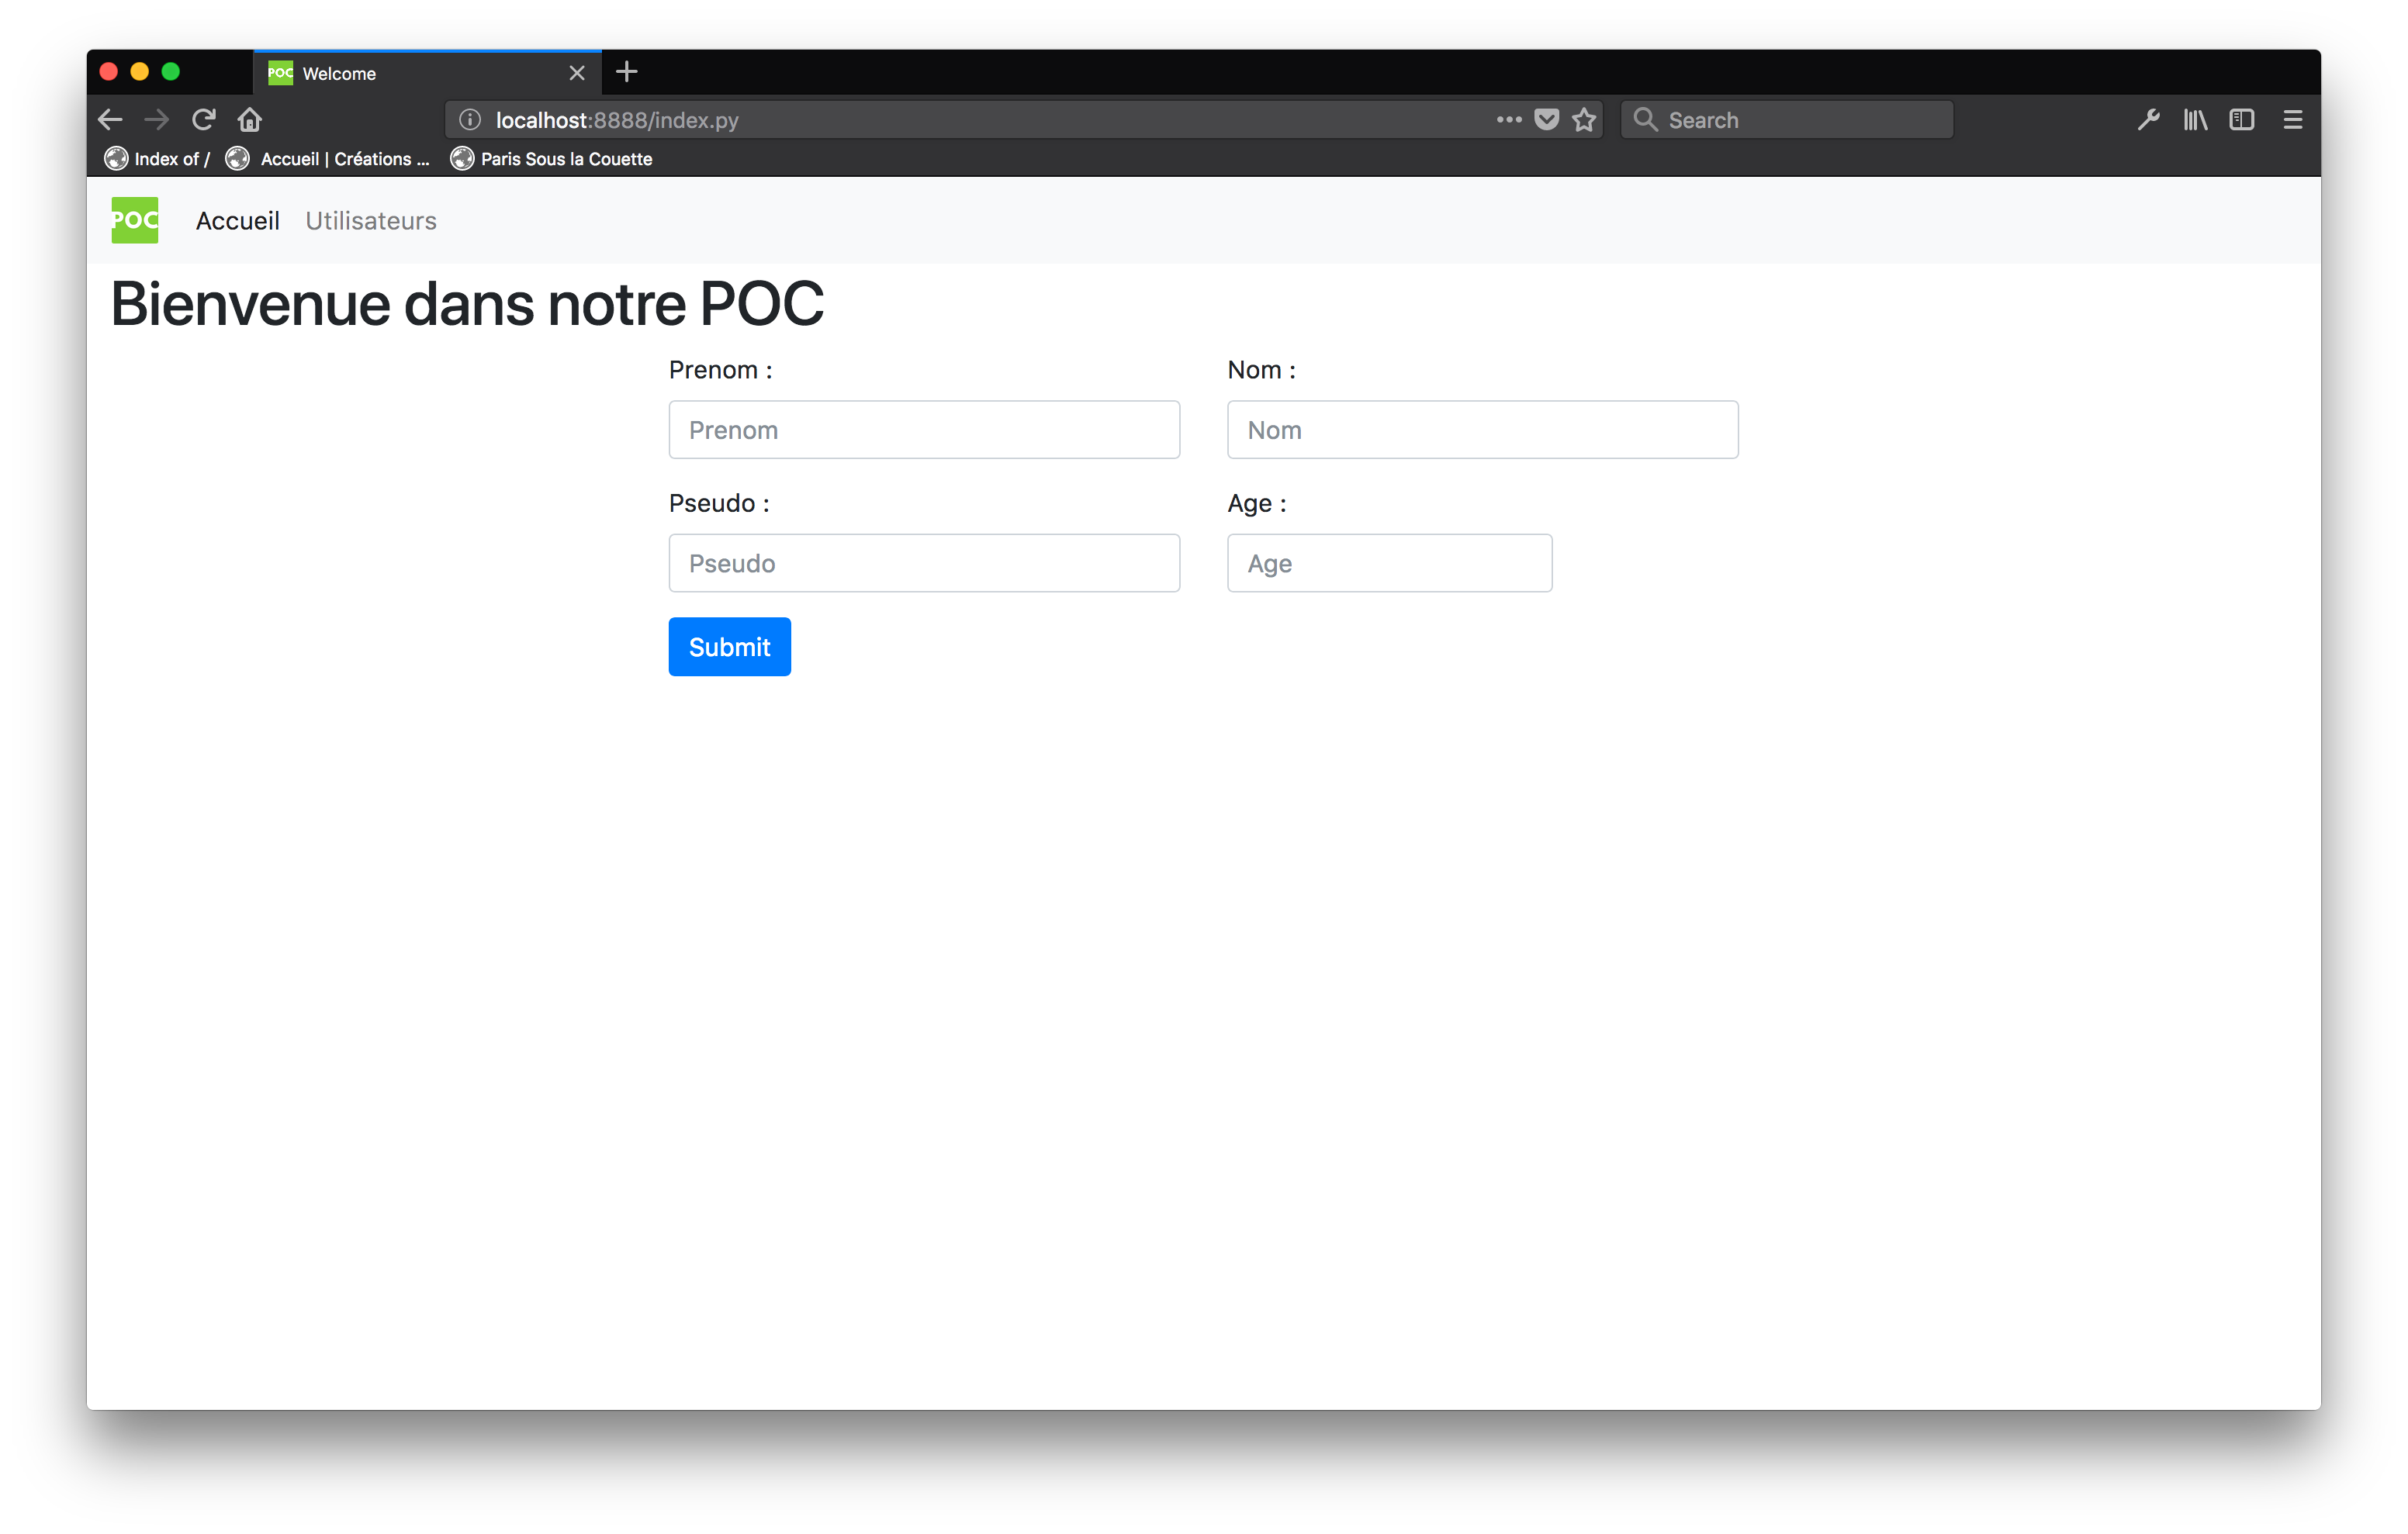
\includegraphics[width=15cm]{images/index.png}
\centering
\end{figure}
\begin{figure}[H]
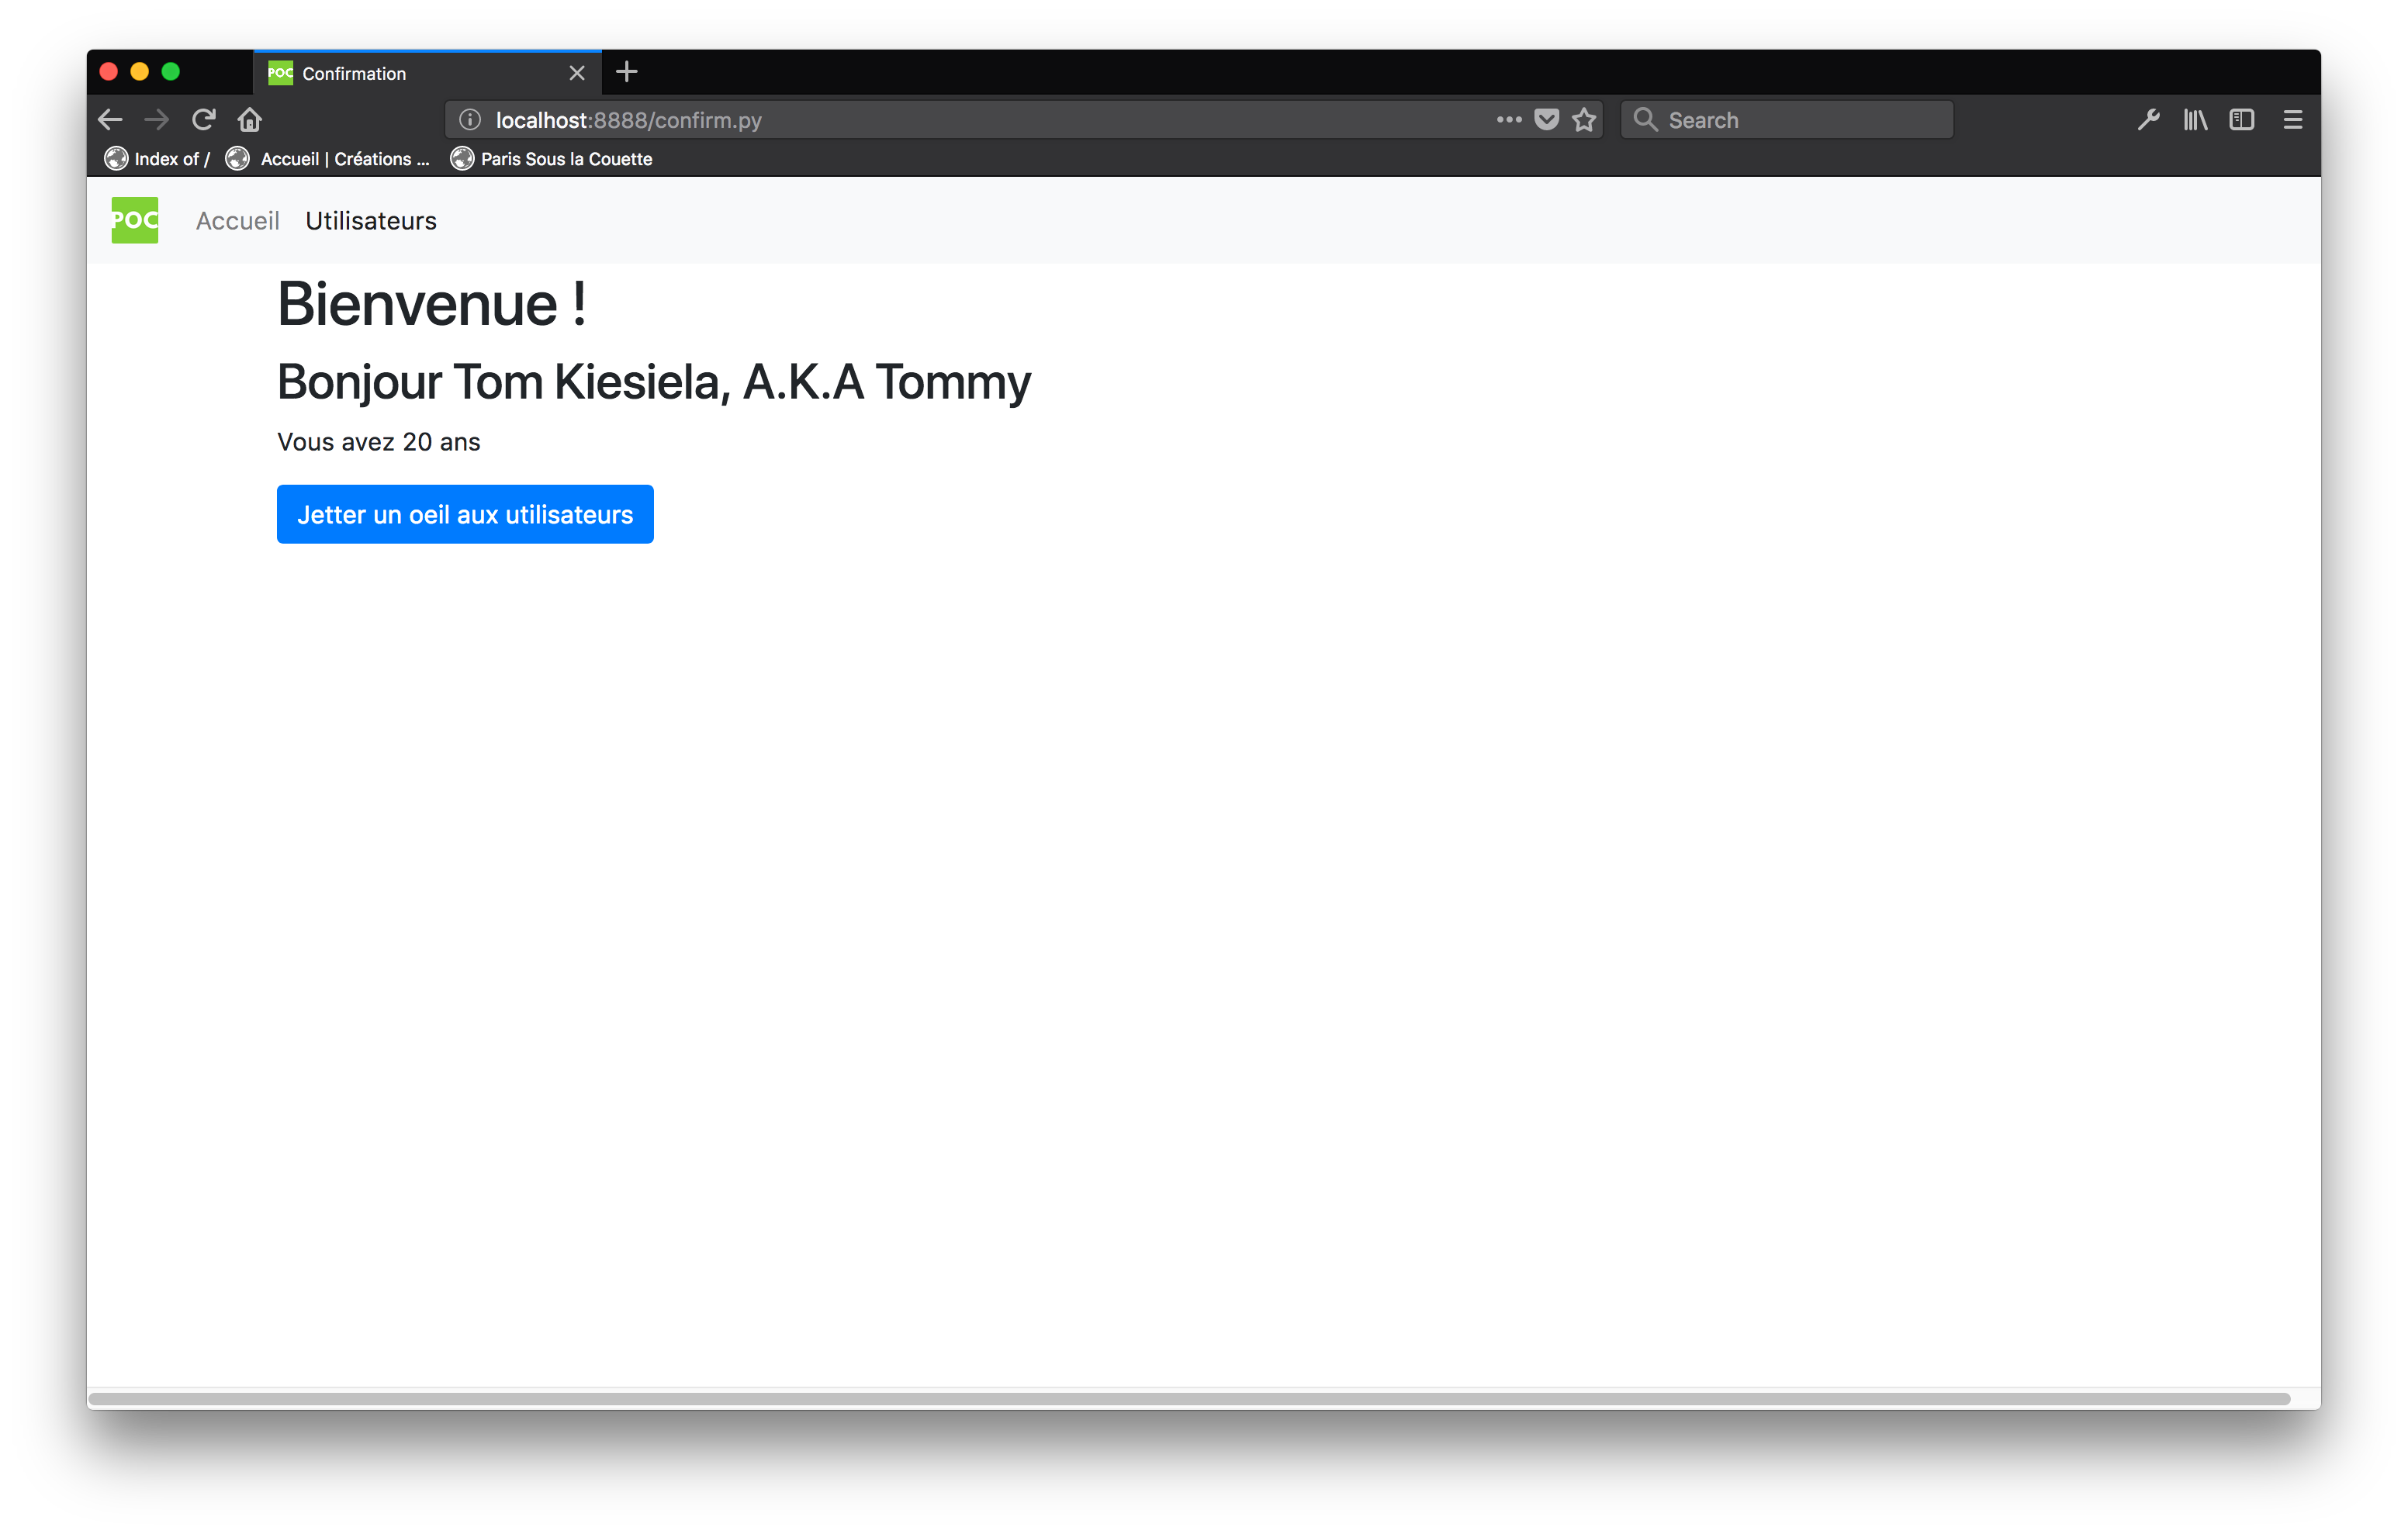
\includegraphics[width=15cm]{images/confirm.png}
\centering
\end{figure}
\begin{figure}[H]
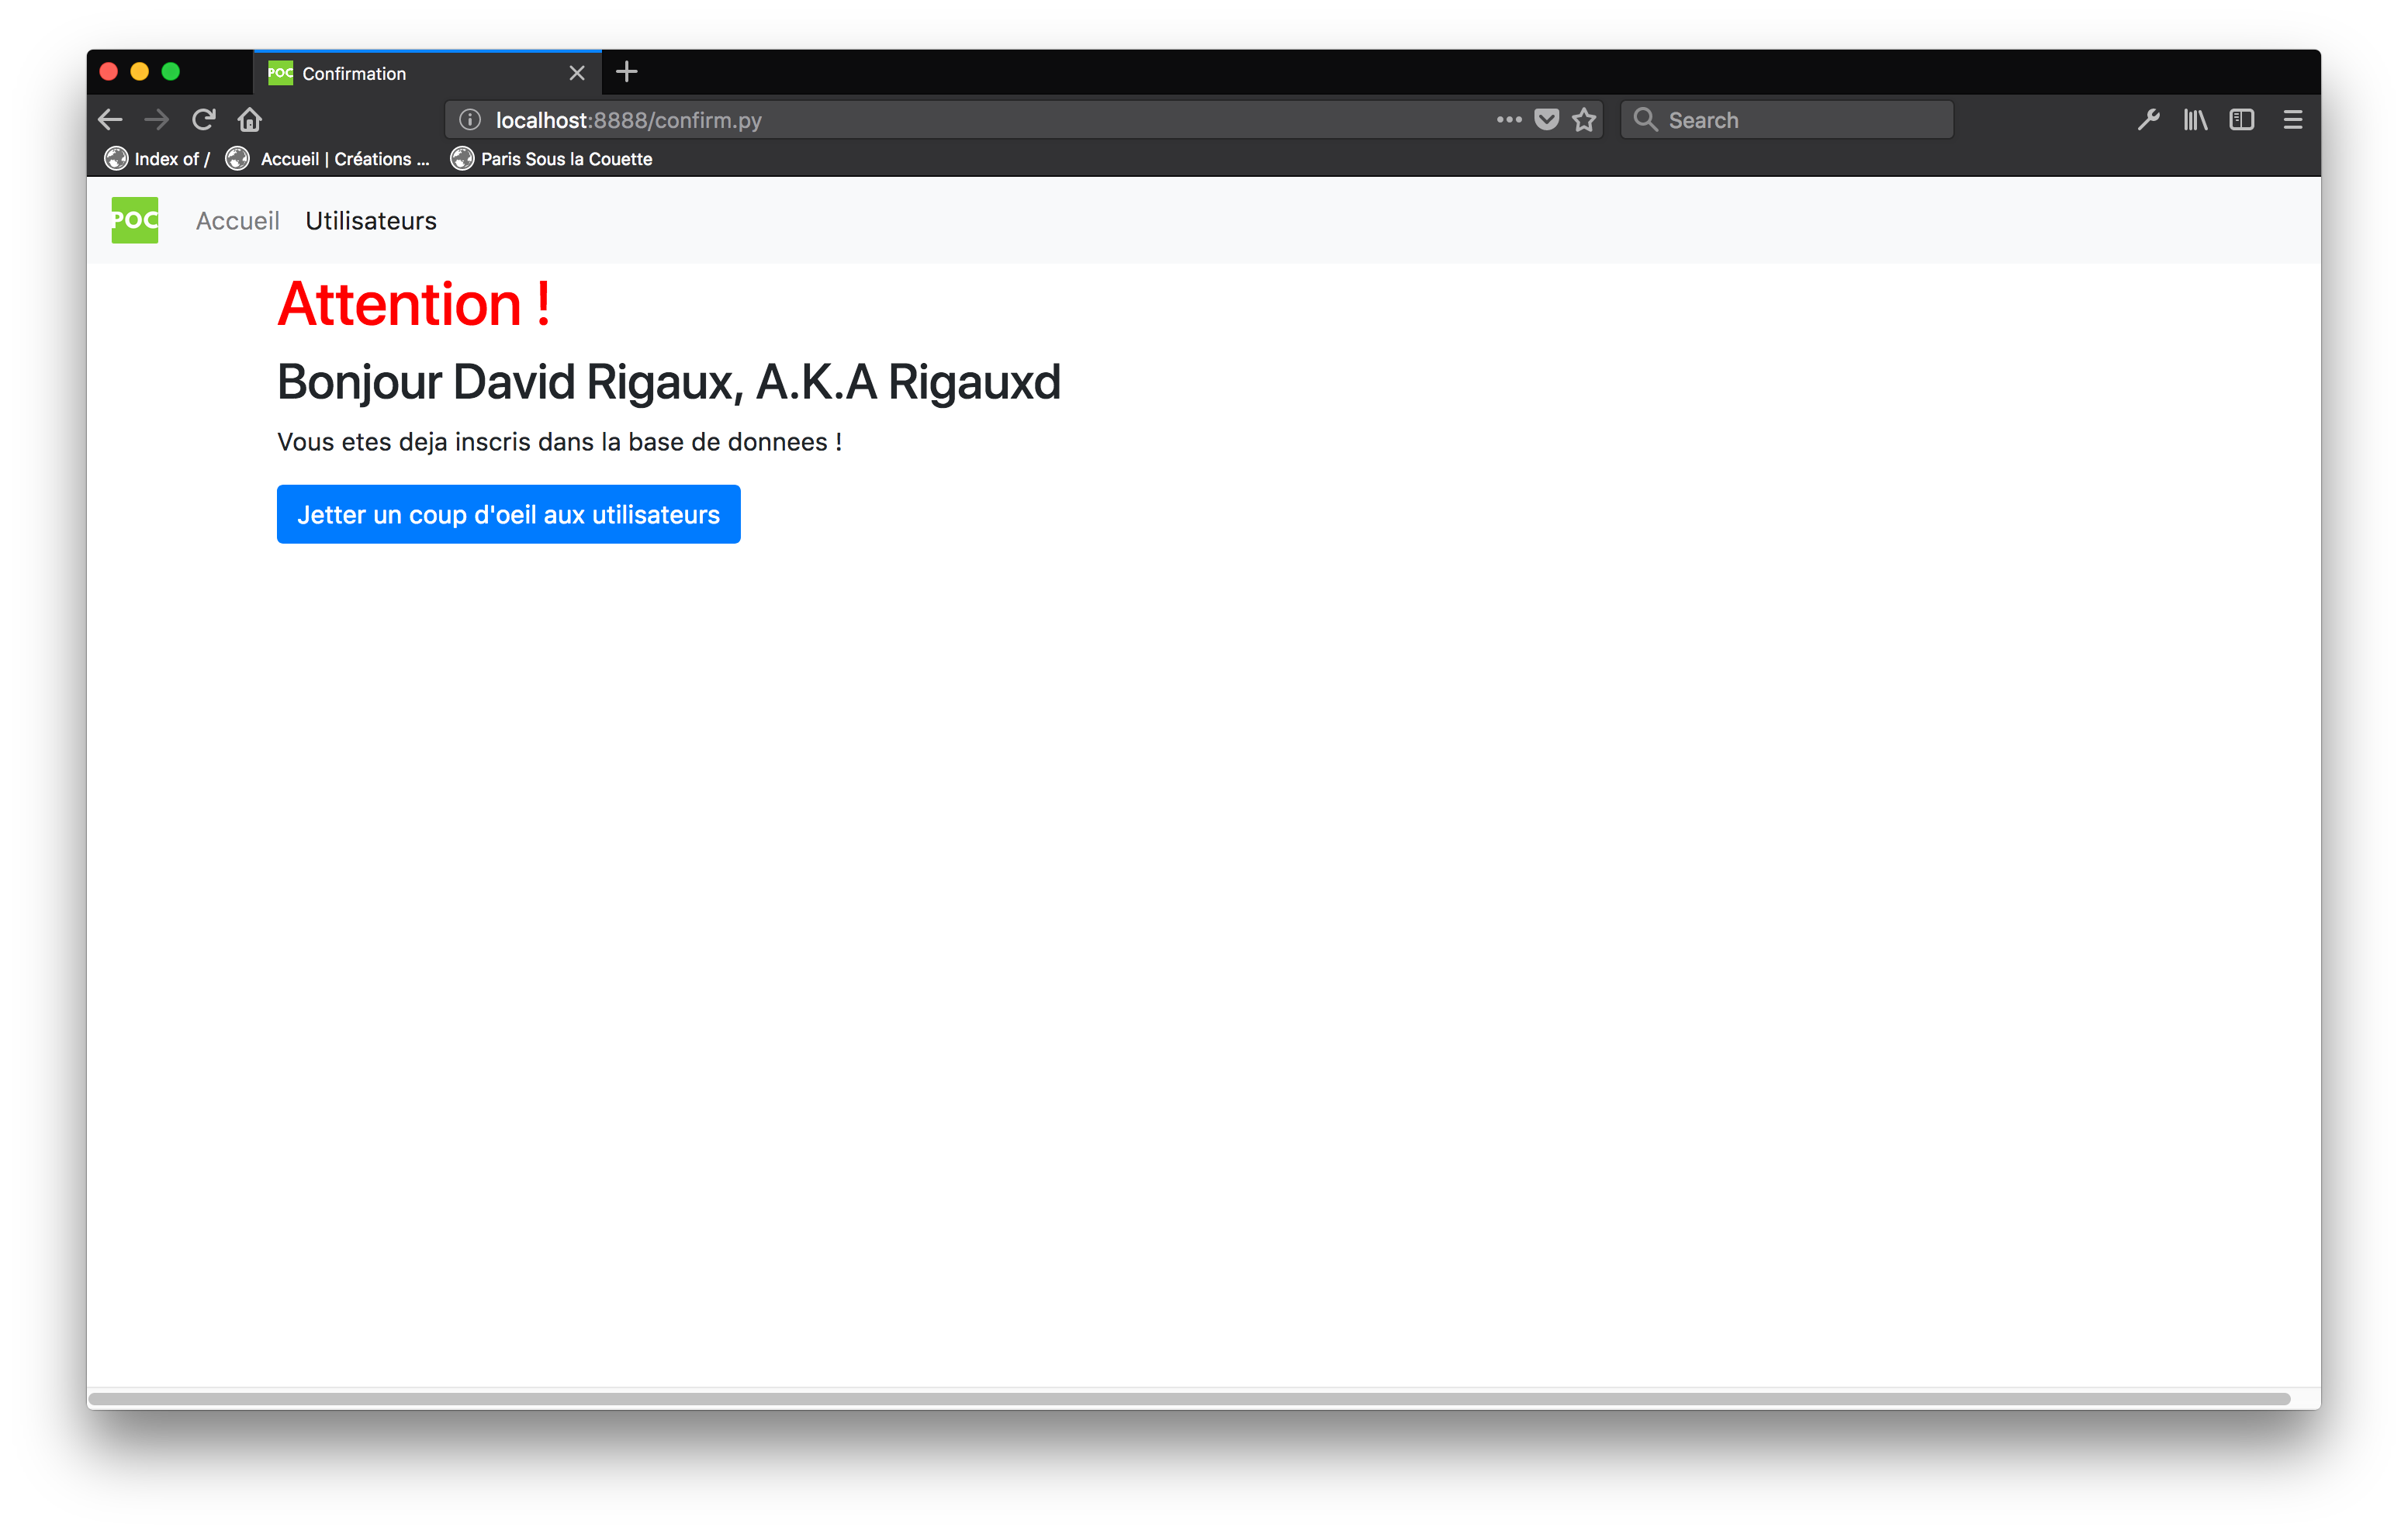
\includegraphics[width=15cm]{images/nonValide.png}
\centering
\end{figure}
\begin{figure}[H]
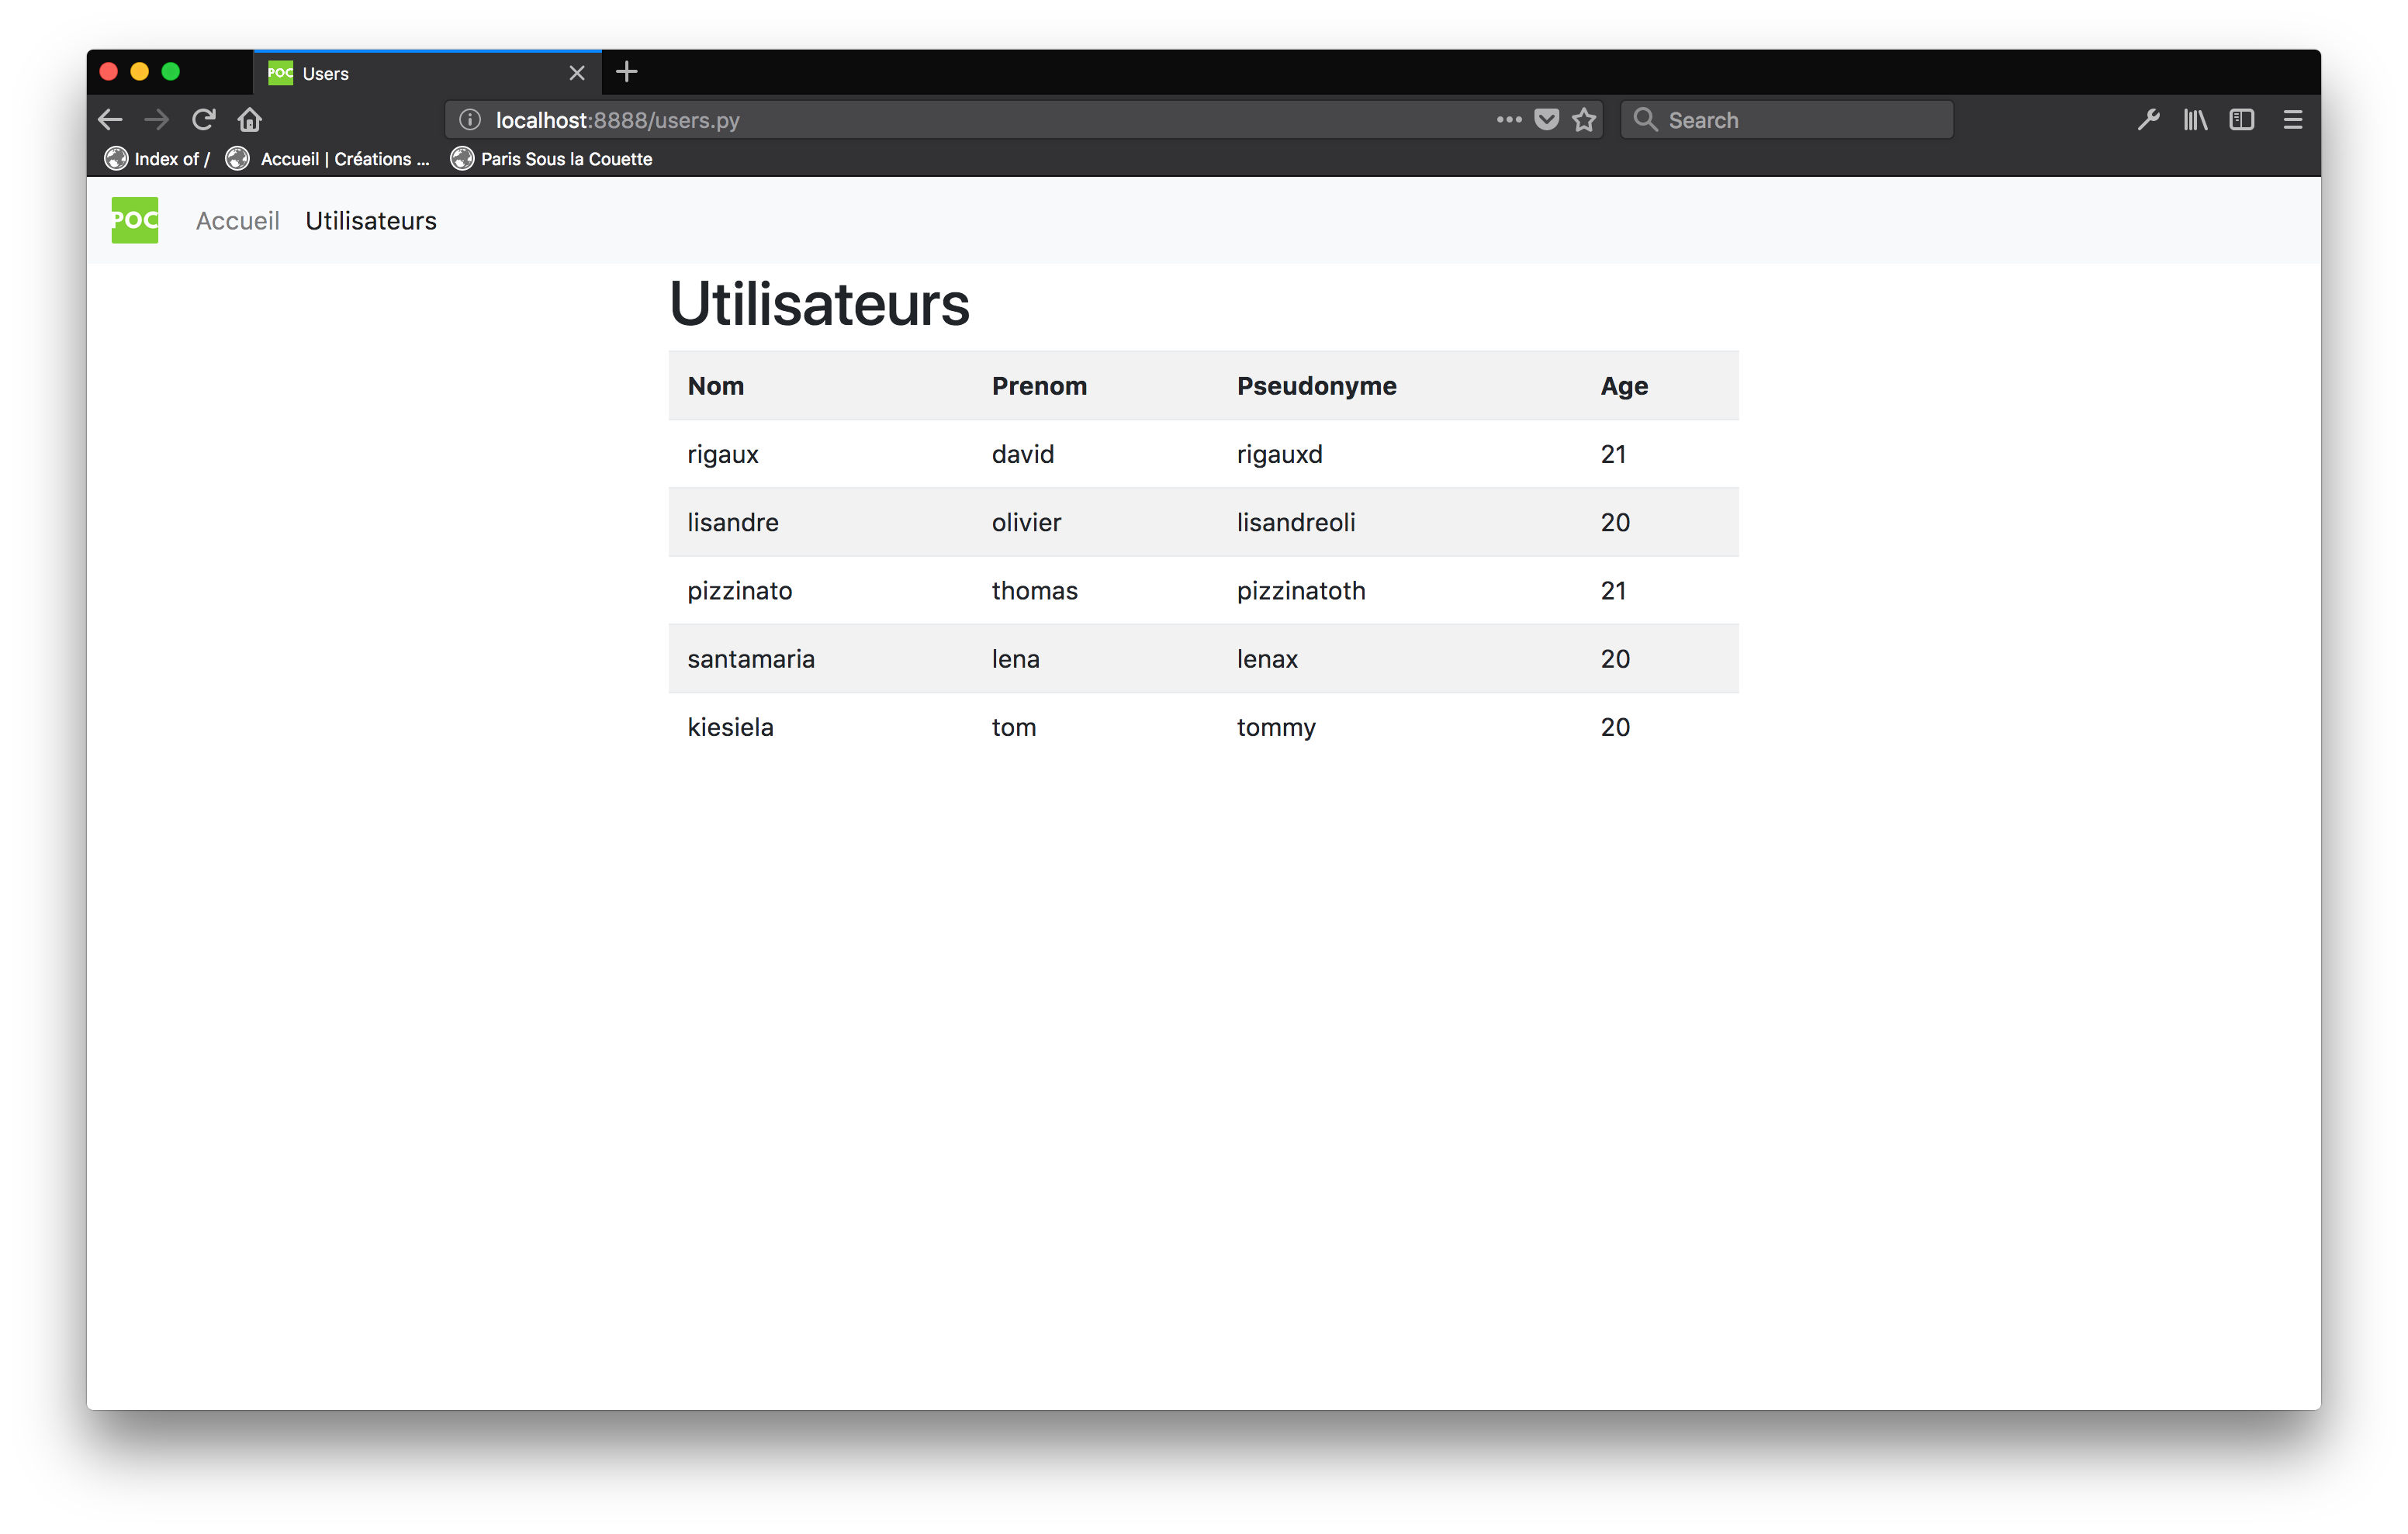
\includegraphics[width=15cm]{images/users.png}
\centering
\end{figure}

\section{Bilan Personnels}
\subsection{Thomas PIZZINATO}
Le but d'apprendre le python web via un projet était une bonne idée. Malheureusement, la communication et l'apprentissage ont été mal exprimés. \par
D'une part au début nous devions faire un POC en deux semaines avec le framework que nous désirions et ce mercredi on nous dit de faire en CGI alors que nous avions commencé Django. Nous avons donc du tout changer et se retrouver au dernier moment pour tout revoir ensemble et changer avec cette déconvenue au dernier moment. \par
D'autre part, nous n’avons eu aucune info sur le framework à utiliser, quels sites conseillés ou même un cours pour apprendre. Ce que j'ai trouvé dommage. \par
Mais grâce à ce projet, j'ai pu travailler auprès d'un bon groupe avec qui l'ambiance de travail et de non-travail était parfaite. 
Et apprendre un nouveau langage est toujours enrichissant !
\subsection{Olivier LISANDRE}
Au départ, nous n’avions pas bien cerné le sujet de ce travail. Nous pensions que nous devions utiliser un Framework et nous avions décidé d’utiliser Django. Nous avons donc durant la première semaine étudié de notre côté pour apprendre à utiliser cet outil.  Lors de la deuxième séance, nous nous sommes concertés pour trouver un projet à réaliser. \par
Cependant, nous avons appris à la fin de cette séance que nous n’avions pas le droit d’utiliser un Framework. Nous devions seulement utiliser du Python. Nous avons donc décidé de regarder rapidement chacun de notre côté comment utiliser le Python pour faire un formulaire en Web.\par
J’ai essayé de mon côté de créer un formulaire en python et une petite base de données.
Le lendemain, nous nous sommes retrouvés pour mettre en commun nos recherches et commencer à élaborer le rendu final. Après cette entrevue, nous avions enfin un rendu acceptable. \par
Au cours de ce projet j’ai appris à utiliser Python, même si je ne suis pas encore à l’aise avec le langage. J’ai aussi revu des notions en HTML et appris à les appliquer à un programme python. Et même si cela ne faisait pas partie des consignes de travail, j’ai appris les bases de l’utilisation de django, ce qui m’aidera pour mes projets futurs.
\subsection{Ismaël L'HOSTE}
Au lancement du projet, nous étions un groupe avec seulement une personne qui connaissait assez bien le python, nous étions donc lâchés dans l’inconnu. J’ai donc alors décidé de me lancer dans la création d’un petit site perso à l’aide de Django. Ce qui fut une rude épreuve pour moi, j’ai donc persévéré sur cette voie pour enfin arriver à un résultat acceptable. C’est alors que le professeur encadrant nous a annoncé qu’il ne fallait pas utiliser Django. Nous sommes donc repartis de loin, avec l’intention d’apprendre le python chacun de son côté, pour cela nous avons développé notre site séparément et avons finalement décidé de vous rendre le plus abouti.
\subsection{David RIGAUX}
Pour ma part, j'avais déjà codé en Python pour diverses raisons. Sachant qu'au tout début du projet on nous avait simplement dit de faire une application simple en Python Web. Nous nous sommes tous mis à faire des recherches pour savoir comment s'y prendre, mais nous n'avions pas trouvé grand-chose à part du développement web avec framework, comme Django. On s'était donc mis d'accord de commencer à apprendre le Django. La semaine d'après, à 15 minutes de la fin Monsieur George est venu nous dire qu'il ne fallait pas utiliser le Framework Django, mais qu'il faudrait jeter un coup d'œil à CGI. \\
Nous nous sommes donc tous lancés dans l'autoformation et à la recherche de pistes pour apprendre le CGI. Nous avons alors tous commencé à développer de notre côté puis finalement nous avons tout mis en commun. J'avais commencé à faire un formulaire et jouer avec les différentes possibilités de développement grâce au langage Python. J'ai trouvé ce projet intéressant même si nous avions était mal mis au courant dès le début, cela était très intéressant. Au final, nous avons réussi à faire quelque chose de correct sachant le peu de temps qu'on avait. 
\section{Conclusion}

Au cours de ce projet, nous avons appris à utiliser le Python. Même si certains d'entre nous connaissaient les bases du langage, certains n'avaient jamais utilisé le Python. Mais c'était la première fois que nous utilisions du Python pour faire du développement Web. 
De plus, nous avons pu réutiliser nos acquis en HTML. Ce qui nous sera toujours utile.

Ce projet nous a permis de voir d'autre possibilité pour faire du développement. Nous pouvons maintenant faire du développement avec du PHP/SQL ou avec du Python. Ce qui nous donne plus de flexibilité et augmente nos possibilités.

\end{document}
